\documentclass[a4paper, 14pt]{article}
\usepackage[margin=1.6cm]{geometry}
\usepackage[utf8]{inputenc}
\usepackage{minted}
\usepackage[russian]{babel}
\usepackage{amsmath}
\usepackage{graphicx}
\usepackage{changepage}
\usepackage{hyperref}
\usepackage{cases}
\usepackage{tikz-timing}[2017/12/20]
\usepackage{relsize}
\usepackage{booktabs}
\usepackage{gensymb}
\usetikzlibrary {arrows.meta}
\pagestyle{empty}

\hypersetup{
	linkbordercolor = {1 1 1}
}

\usepackage{tikz-timing}[2009/05/15]
\usepackage{multicol}
\usepackage[T2A]{fontenc}
\usepackage{pgfplots}
%\usepackage[left=2.5cm, right=1.5cm, vmargin=2.5cm]{geometry}
\setlength\parindent{0pt} % Удалить отступы из параграфов.

\usepackage{listings}
\usepackage{caption}
\DeclareCaptionFont{white}{\color{white}} % Текст заголовка.
\DeclareCaptionFormat{listing}{\colorbox{gray}{\parbox{\textwidth}{#1#2#3}}}
\captionsetup[lstlisting]{format=listing,labelfont=white,textfont=white}
\renewcommand\labelenumi{\theenumi)}
\setlength\parindent{24pt}



\begin{document}
\lstset{
	language=java,                 % Выбор языка для подсветки (здесь это java).
	basicstyle=\small\sffamily,    % Размер и начертание шрифта для подсветки кода.
	numbers=left,                  % Где поставить нумерацию строк (слева\справа).
	numberstyle=\tiny,             % Размер шрифта для номеров строк.
	stepnumber=1,                  % Размер шага между двумя номерами строк.
	firstnumber=1,
	numberfirstline=true
	numbersep=5pt,                 % Как далеко отстоят номера строк от подсвечиваемого кода.
	backgroundcolor=\color{white}, % Цвет фона подсветки - используем \usepackage{color}.
	showspaces=false,              % Показывать или нет пробелы специальными отступами.
	showstringspaces=false,        % Показывать или нет пробелы в строках.
	showtabs=false,                % Показывать или нет табуляцию в строках.
	frame=single,                  % Рисовать рамку вокруг кода.
	tabsize=2,                     % Размер табуляции по умолчанию равен 2 пробелам.
	captionpos=t,                  % Позиция заголовка вверху [t] или внизу [b].
	breaklines=true,               % Автоматически переносить строки (да\нет).
	breakatwhitespace=false,       % Переносить строки только если есть пробел.
	escapeinside={\%*}{*)}         % Если нужно добавить комментарии в коде.
}

\begin{titlepage}
	\center

	ФЕДЕРАЛЬНОЕ ГОСУДАРСТВЕННОЕ АВТОНОМНОЕ ОБРАЗОВАТЕЛЬНОЕ УЧРЕЖДЕНИЕ ВЫСШЕГО ОБРАЗОВАНИЯ\linebreak
	«Санкт-Петербургский политехнический университет Петра Великого»\\[1cm]
	\textsc{\Large Институт компьютерных наук и технологий}\\
	\textsc{\large Высшая школа программной инженерии}\\[1.5cm]

	{ \huge \bfseries КУРСОВАЯ РАБОТА	\\
	\Large \mdseries ОПРЕДЕЛЕНИЕ РАССТОЯНИЯ ДО ОБЪЕКТА ПУТЕМ УЛЬТРАЗВУКОВОГО ИЗМЕРЕНИЯ С ПОМОЩЬЮ HC-SR04 \\
	\large по дисциплине <<Микропроцессорные системы>>}\\

	\begin{figure}[H]
		\centering
		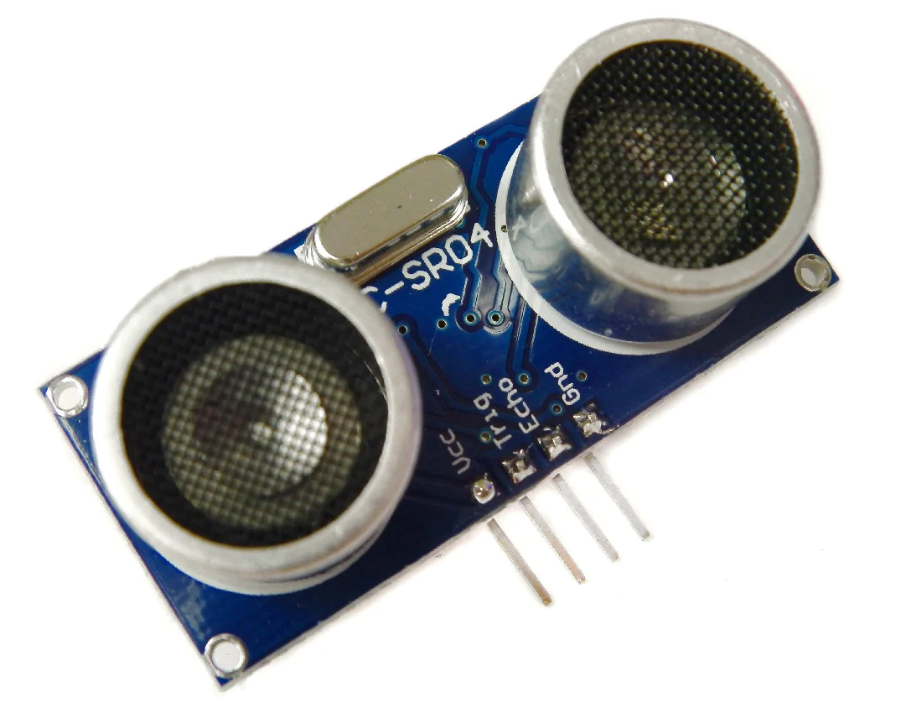
\includegraphics[width=12cm]{screenshots/1.png}\\[2.0cm]
	\end{figure}

	\begin{multicols}{2}
		\begin{flushright} \large

			{Выполнили студенты группы: 3530904/00104:}\\
			{\phantom{qwe}}\\
			{\phantom{qwe}}\\
			{\phantom{qwe}}\\
			{\phantom{qwe}}\\

			{Преподаватель:\\}

		\end{flushright}
		\begin{flushright}

			{Пятизбянцев И. А.}\\
			{Мурзаканов И. М.}\\
			{Поздняков А. А.}\\
			{Почернин В. С.}\\
			{Шиляев В. С.}\\[0.5cm]


			Круглов С. К.\\

		\end{flushright}
	\end{multicols}

	\flushright{
	{\phantom{qwe}}\\[1.5cm]
	{\today}\\
	}
	\centering{
		Санкт-Петербург\\
		2022
	}

	\vfill
\end{titlepage}

\Large
\tableofcontents
\newpage

\section{Условие задачи}

Поставленная задача: разработать и собрать систему на базе платы с процессором ARM, которая позволит измерить расстояние до объекта с помощью ультразвукового датчика.

\newpage
\section{Используемое оборудование}

При выборе основной платы была выбрана Raspberry Pi. В нашем случае в качестве операционной системы использовался Raspbian OS - родной дистрибутив для платы. Таким образом на данной плате получилось не только запустить проект, но и вывести результаты благодаря подключению по SSH.

Ниже представлены \textbf{технические характеристики}:

\begin{itemize}
	\item \textbf{Процессор}: Quad core Cortex-A72 (ARM v8) 64-bit SoC @ 1.5GHz;
	\item \textbf{Оперативная память}: 4GB LPDDR4-2400 SDRAM;
	\item \textbf{Цифровой видеовыход}: HDMI;
	\item \textbf{Композитный выход}: 3.5 мм (4 pin);
	\item \textbf{USB порты}: USB 2.0 x4;
	\item \textbf{Сеть}: WiFi 802.11n, 10/100 Мб RJ45 Ethernet;
	\item \textbf{Bluetooth}: Bluetooth 4.1, Bluetooth Low Energy;
	\item \textbf{Разъем дисплея}: Display Serial Interface (DSI);
	\item \textbf{Карта памяти}: MicroSD;
	\item \textbf{Порты ввода-вывода}: 40;
	\item \textbf{Модуль}: HC-SR04 Ultrasonic Range Sensor;
	\item \textbf{Радиодетали}:
	      \begin{itemize}
		      \item $1k\Omega$ резистор;
		      \item $2k\Omega$ резистор;
		      \item Соединительные провода;
	      \end{itemize}
\end{itemize}

\newpage
\section{Ультразвуковые датчики расстояния}

\subsection{Общее описание}

\begin{figure}[H]
	\centering
	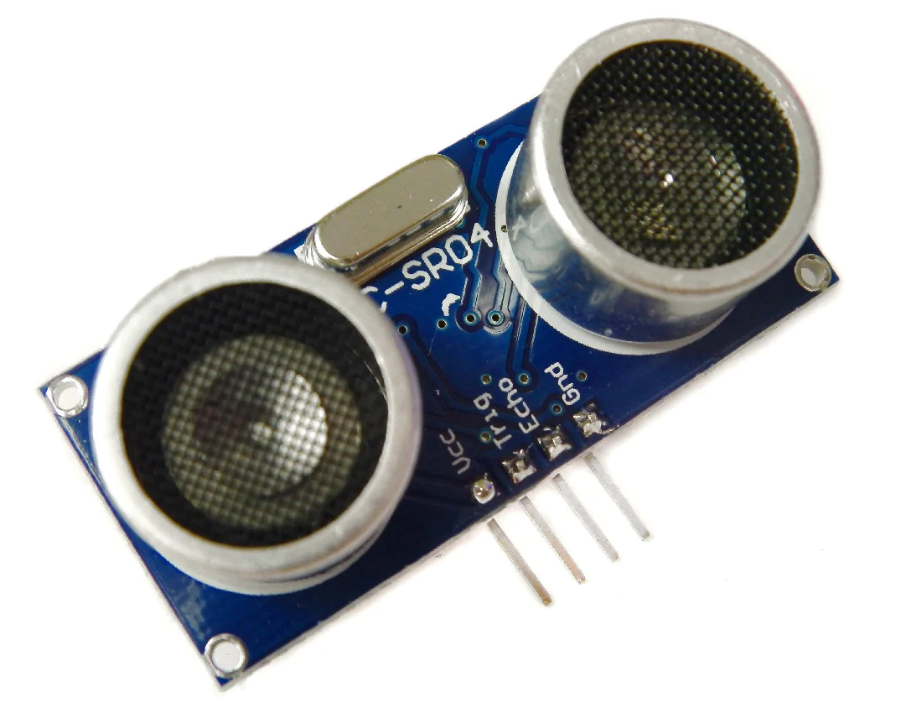
\includegraphics[width=15cm]{screenshots/1.png}\\
	\caption{Ультразвуковой датчик HC-SR04}
\end{figure}

Звук состоит из колеблющихся волн в среде (например, в воздухе), высота звука которых определяется близостью этих волн друг к другу и называется \textbf{частотой}. Человеческому уху слышна только часть звукового спектра - диапазон частот звуковых волн, определяемый как \textbf{акустический диапазон}.

Очень низкочастотный звук ниже акустического диапазона определяется как \textit{инфразвук}, выше - как \textit{ультразвук}. Ультразвуковые датчики предназначены для определения близости или расстояния до объекта с помощью отражения ультразвука, подобно радару. Они используют механизм расчета времени, необходимого для отражения ультразвуковых волн между датчиком и твердым объектом.

Ультразвук в основном используется, потому что он не слышим для человеческого уха и относительно точен на коротких расстояниях. Можно, конечно, использовать для этой цели акустический звук, однако, в таком случае мы получим менее точные измерения и раздражающее устройство, которое будет издавать неприятные звуки раз в секунду.

Базовый ультразвуковой датчик состоит из одного или нескольких ультразвуковых динамиков, приемника и схемы управления.

Динамики излучают высокочастотный ультразвук, который отражается от любых близлежащих твердых предметов. Часть этого ультразвукового шума отражается и обнаруживается приемником на датчике. Затем этот обратный сигнал обрабатывается схемой управления для вычисления разницы во времени между передаваемым и принимаемым сигналом.

Это время можно впоследствии использовать вместе с некоторыми умными математическими вычислениями для расчета расстояния между датчиком и отражающим объектом.

\subsection{Описание HC-SR04}

Ультразвуковой датчик \textit{HC-SR04}, который мы будем использовать для Raspberry Pi имеет четыре контакта:

\begin{itemize}
	\item Заземление (GND);
	\item Выход эхо-импульса (ECHO);
	\item Вход триггерного испульса (TRIG);
	\item Источник питания 5В (VCC);
\end{itemize}

Мы питаем модуль с помощью VCC, заземляем его с помощью GND и используем наш Raspberry Pi для отправки входного сигнала на TRIG, который запускает датчик для отправки ультразвукового импульса.

Пульсовые волны отражаются от любых близлежащих объектов, а некоторые отражаются обратно к датчику. Датчик обнаруживает эти возвратные волны и измеряет время между триггером и возвратным импульсом, а затем отправляет сигнал 5В на выход ECHO.

ECHO будет <<низким>> (0В) до тех пор, пока датчик не сработает, когда получит TRIG импульс. Как только триггерный импульс будет обнаружен - ECHO устанавливается на <<высокий уровень>> (5В) на время этого импульса (т. е. пока выпущенный звуковой сигнал не вернется обратно). Длительность импульса - это полное время между отправкой датчиком ультразвукового импульса и обнаружением обратного импульса приемником датчика. Поэтому наш Python скрипт должен будет измерить длительность импульса, а затем вычислять расстояние, исходя из этого.

Однако, существует трудность. Дело в том, что выходной сигнал датчика ECHO на HC-SR04 рассчитан на 5В, в то время, как входной контакт Raspberry Pi GPIO рассчитан на 3.3В. Отправка сигнала 5В на этот незащищенный входной порт может повредить контакты GPIO.

Нам понадобится небольшая схема делителя напряжения, состоящая из двух резисторов, чтобы снизить выходное напряжение датчика до уровня, с которым может справиться Raspberry Pi.

\newpage
\subsection{Спецификация HC-SR04}

\begin{table}[h!]
	\centering
	\begin{tabular}{ll}
		\toprule
		\textbf{Параметр}           & \textbf{Значение}                                           \\
		\midrule
		Рабочее напряжение          & \(3,3 \text{ В} \sim 5 \text{ В}\)                          \\
		Сила тока покоя             & \(<2\text{ мА}\)                                            \\
		Рабочая сила тока           & \(15\text{ мА}\)                                            \\
		Рабочая частота             & \(40\text{ кГц}\)                                           \\
		Рабочий диапазон и точность & \(2 \text{ см} \sim 400 \text{ см} \pm 3 \text{ мм}\)       \\
		Чувствительность            & \(-65 \text{ дБ}\) минимум                                  \\
		Звуковое давление           & \(112 \text{ дБ}\)                                          \\
		Эффективный угол            & \(15 \degree\)                                              \\
		Соединение                  & 4-контактный разъём                                         \\
		Размеры                     & \(45 \text{ мм} \times 20 \text{ мм} \times 15 \text{ мм}\) \\
		Вес                         & \(9 \text{ г}\)                                             \\
		\bottomrule
	\end{tabular}
	\caption{Спецификация датчика}
\end{table}

В элементах датчика используются пьезоэлектрические кристаллы.
Когда на них подаётся ток, они колеблются на высоких частотах.
Пьезоэлектрические кристаллы генерируют электрический сигнал, когда
ультразвуковая волна возвращается к поверхности датчика.

\begin{figure}[h!]
	\centering
	\scalebox{1.2}{
		\tikzset{
			timing/rowdist = 1.4cm,
			timing/font = {\small},
			timing/yunit = 0.8cm,
			fontscale/.style = {font=\relsize{#1}}
		}
		\tikztimingsetwscale{3.0}
		\begin{tikztimingtable}
			Триггерный вход & LH7LlHL \\
			Ультразвук & 5l [!wscale=\wscale/6!] 16{C} [!wscale=\wscale*6!] 6L[!wscale=\wscale/1.5!]l \\
			Эхо-выход & 5l [!wscale=\wscale/6!] 16L [!wscale=\wscale*6!] 3Hh 5l[!wscale=\wscale/1.5!]l \\
			\extracode
			\begin{pgfonlayer}{background}
				\node [anchor=south, inner sep=0pt, align=center] at (4.5,1.2) [fontscale=-2] {Подаётся импульс \\ на триггер};
				\node [anchor=south, inner sep=0pt, align=left] at (22,-1.5) [fontscale=-2] {Отправляется восемь \\ 40 кГц импульсов};
				\node [anchor=south, inner sep=0pt, align=center] at (21,-4.5) [fontscale=-2] {Время между выпуском ультразвукового \\ импульса и его возвращением};
				\node [anchor=south, inner sep=0pt, align=center, blue] at (8.5,-2.4) [fontscale=-2] {25 мкс};
				\node [anchor=south, inner sep=0pt, align=center, blue] at (4.5,-0.6) [fontscale=-2] {10 мкс};
				\draw[<->, blue] (15.5,-3.2) -- (26,-3.2);
				\draw[|-|, blue] (8,-2) -- (9,-2);
				\draw[|-|, blue] (3,-0.2) -- (6,-0.2);
			\end{pgfonlayer}
		\end{tikztimingtable}
	}
	\caption{Временная диаграмма работы датчика}
\end{figure}

Выше показана временная диаграмма работы датчика.
Чтобы начать замеры, необходимо подать короткий импульс 10 мкс на триггерный контакт.
Модуль отправит пакет из 8 ультразвуковых импульсов и переведёт эхо-выход в высокий уровень. Уровень эхо-выхода вновь станет низким, когда датчик примет отраженный звуковой сигнал.

По интервалу времени между отправкой ультразвуковых импульсов и получением эхо-сигнала можно
рассчитать расстояние.

Рекомендуется использовать цикл измерения дольше 60 мс.

Для наилучших результатов
поверхность объекта для обнаружения должна иметь площадь не менее \(0,5 \text{ м}^2\).

\newpage
\section{Raspberry Pi 4B. GPIO}

\subsection{Описание}

В первую очередь необходимо рассмотреть ключевые особенности этого интерфейса. И самое главное в GPIO Raspberry Pi – это pings (пины). Именно они используются для связи одноплатника с периферией.
В совокупности есть 26 GPIO (портов). Все они являются \textit{цифровыми}.

\begin{figure}[H]
	\centering
	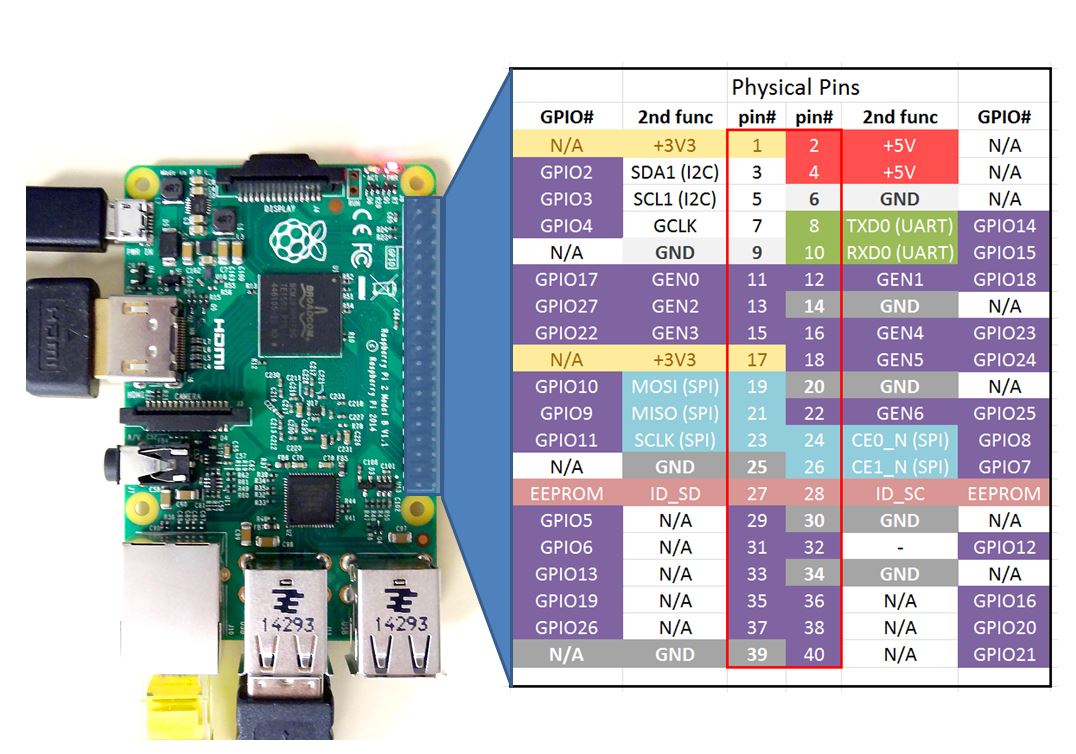
\includegraphics[width=12cm]{screenshots/999.png}\\
	\caption{Расширенная схема GPIO}
\end{figure}

\subsection{Взаимодействие}

Работать с GPIO Raspberry Pi можно практически через любой инструмент. К сегодняшнему дню созданы соответствующие библиотеки почти под все распространенные языки программирования.

Однако мы решили взаимодействовать с данным интерфейсом посредством Python. Это обусловлено, во-первых тем, что для GPIO в Raspbian уже предустановлена соответствующая библиотека для Python, а, во-вторых, этот ЯП является основным для рассматриваемого одноплатника.

Однако при желании, конечно, можно пользоваться и любыми другими инструментами. Найти название библиотек и их описание не составляет никакого труда.

\newpage
\section{Схема устройства}

\subsection{Делитель напряжения}

Делитель напряжения, который мы будем использовать состоит из двух резисторов ($R_1$ и $R_2$), последовательно подключенных к входному напряжению (Vin), которое необходимо уменьшить до нашего выходного напряжения (Vout). В нашей схеме Vin будет ECHO, который нужно уменьшить на Vout (вход GPIO) c 5В до 3.3В.

\begin{figure}[H]
	\centering
	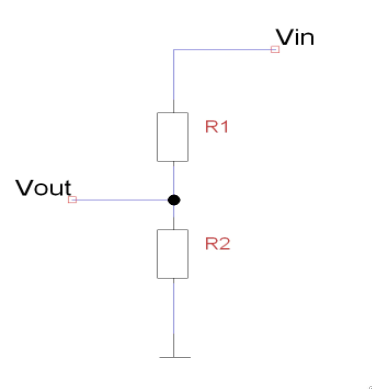
\includegraphics[width=7cm]{screenshots/2.png}\\
	\caption{Схема делителя напряжения}
\end{figure}

В действительности, нам нужно рассчитать только одно значение резистора, так как нам важен коэффициент деления:
$$V_\text{out} = V_\text{in} \times \frac{R_2}{R_1 + R_2}$$

$$\frac{V_\text{out}}{V_\text{in}} = \frac{R_2}{R_1+R_2}$$

Мы знаем наше входное напряжение 5В и требуемое выходное напряжение 3.3В, соответственно, можем использовать любую комбинацию резисторов для достижения снижения. Пусть $R_1 = 1\text{k}\Omega$, тогда получим:
$$\frac{3.3}{5}=\frac{R_2}{1000+R_2}$$

$$0.66=\frac{R_2}{1000+R_2}$$

$$0.66(1000+R_2) = R_2$$

$$660 + 0.66R_2 = R_2$$

$$660 = 0.34R_2$$

$$R_2 \approx 2\text{k}\Omega$$

\subsection{Схема устройства}

Резюмируя вышесказанное, мы можем представить следующую схему проекта:

\begin{figure}[H]
	\centering
	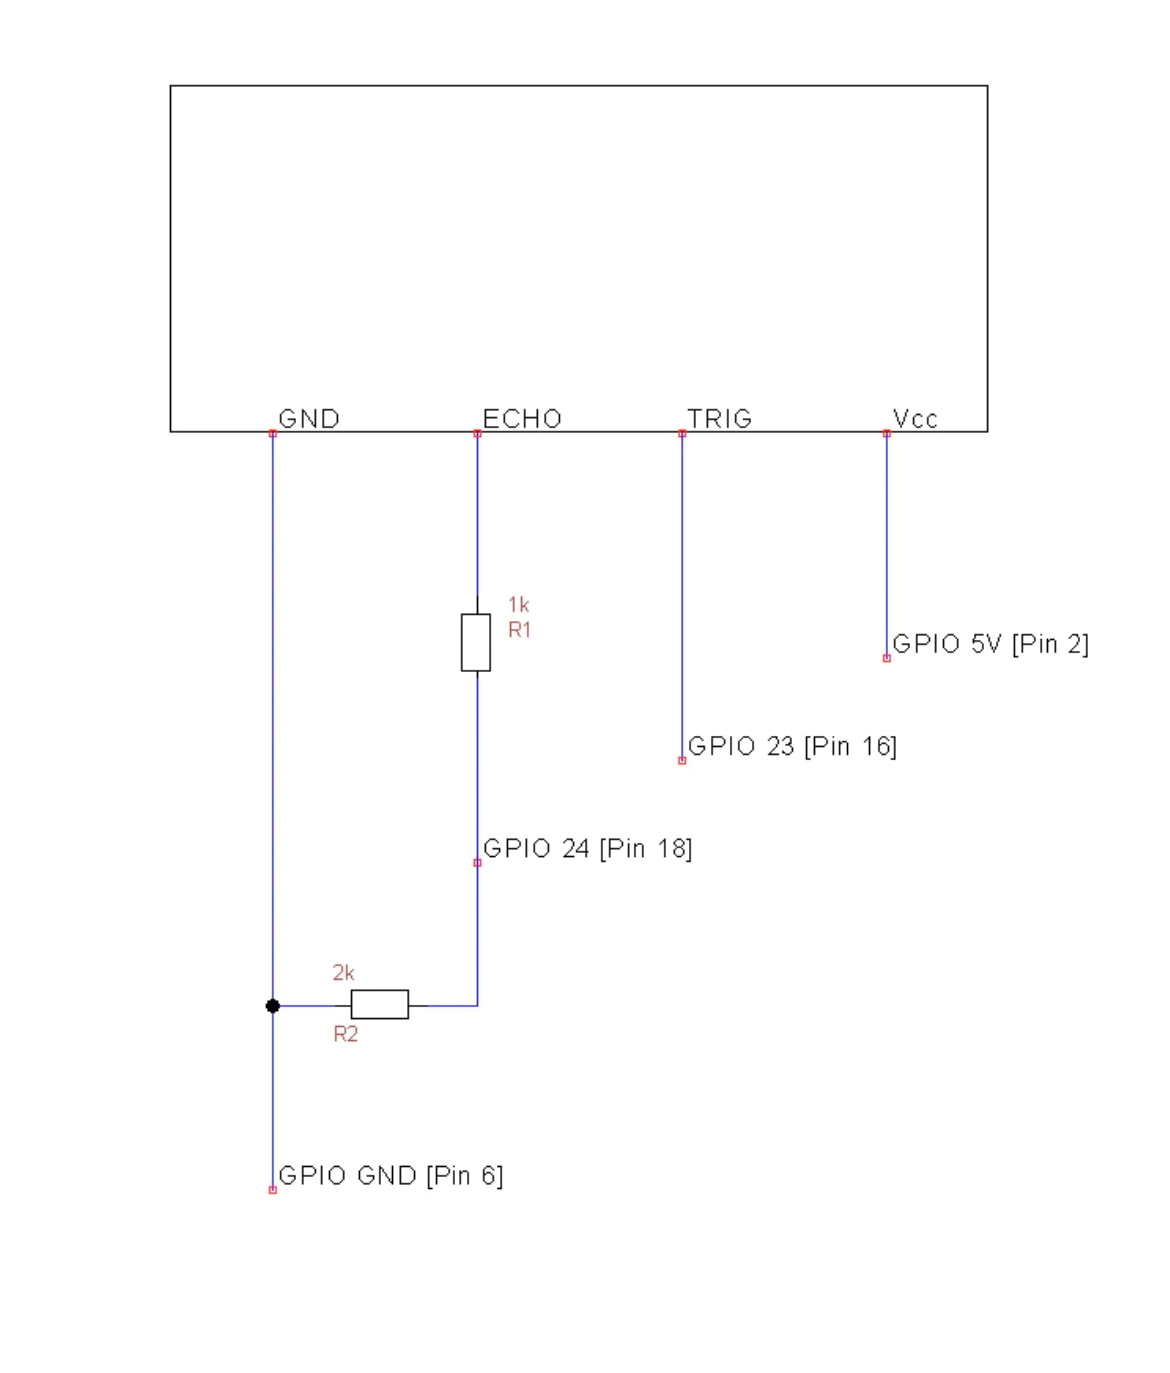
\includegraphics[width=12cm]{screenshots/3.png}\\
	\caption{Схема проекта}
\end{figure}

Еще раз покажем схему в другом виде:

\begin{figure}[H]
	\centering
	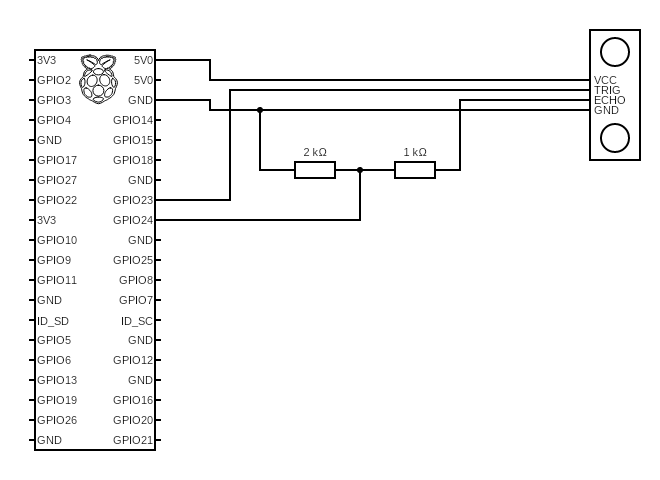
\includegraphics[width=12cm]{screenshots/5.png}\\
	\caption{Более наглядная схема}
\end{figure}

\subsection{Сборка схемы}

Рассмотрим полный алгоритм сборки схемы с использованием макетной платы:

\begin{enumerate}
	\item Первым шагом подключаем перемычки типа <<папа-мама>> в контакты на HC-SR04 следующим образом:
	      \begin{figure}[H]
		      \centering
		      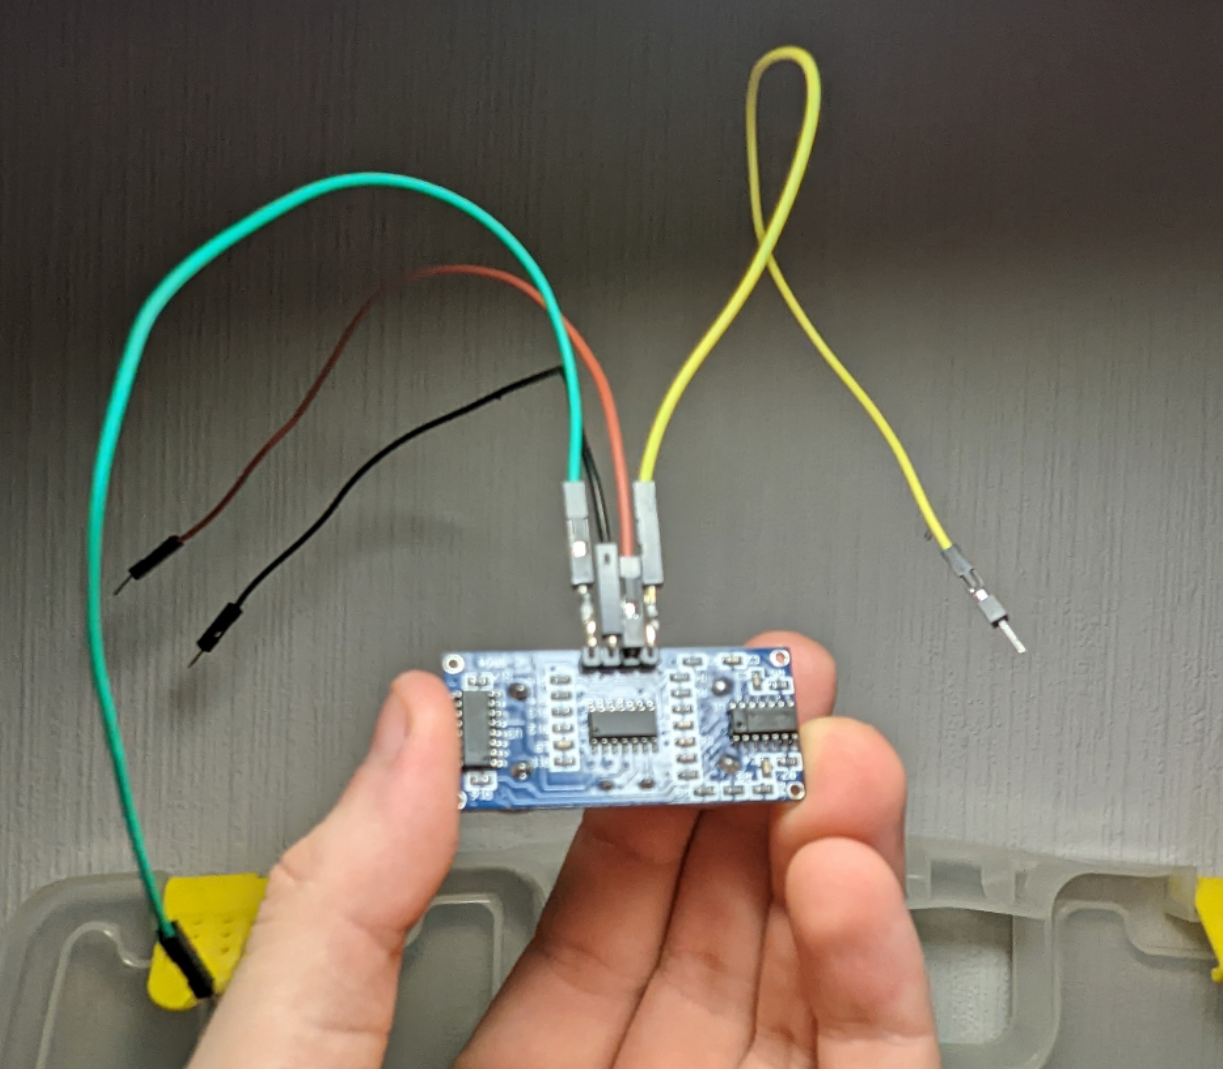
\includegraphics[width=12cm]{screenshots/6.png}\\
		      \caption{Подключение перемычек к HC-SR04}
	      \end{figure}
	\item Подключаем VCC к положительной шине макетной платы и GND к отрицательной шине макетной платы.
	\item Подключаем GPIO 5V к положительной шине макетной платы, а GPIO GND к отрицательной шине макетной платы.
	      \begin{figure}[H]
		      \centering
		      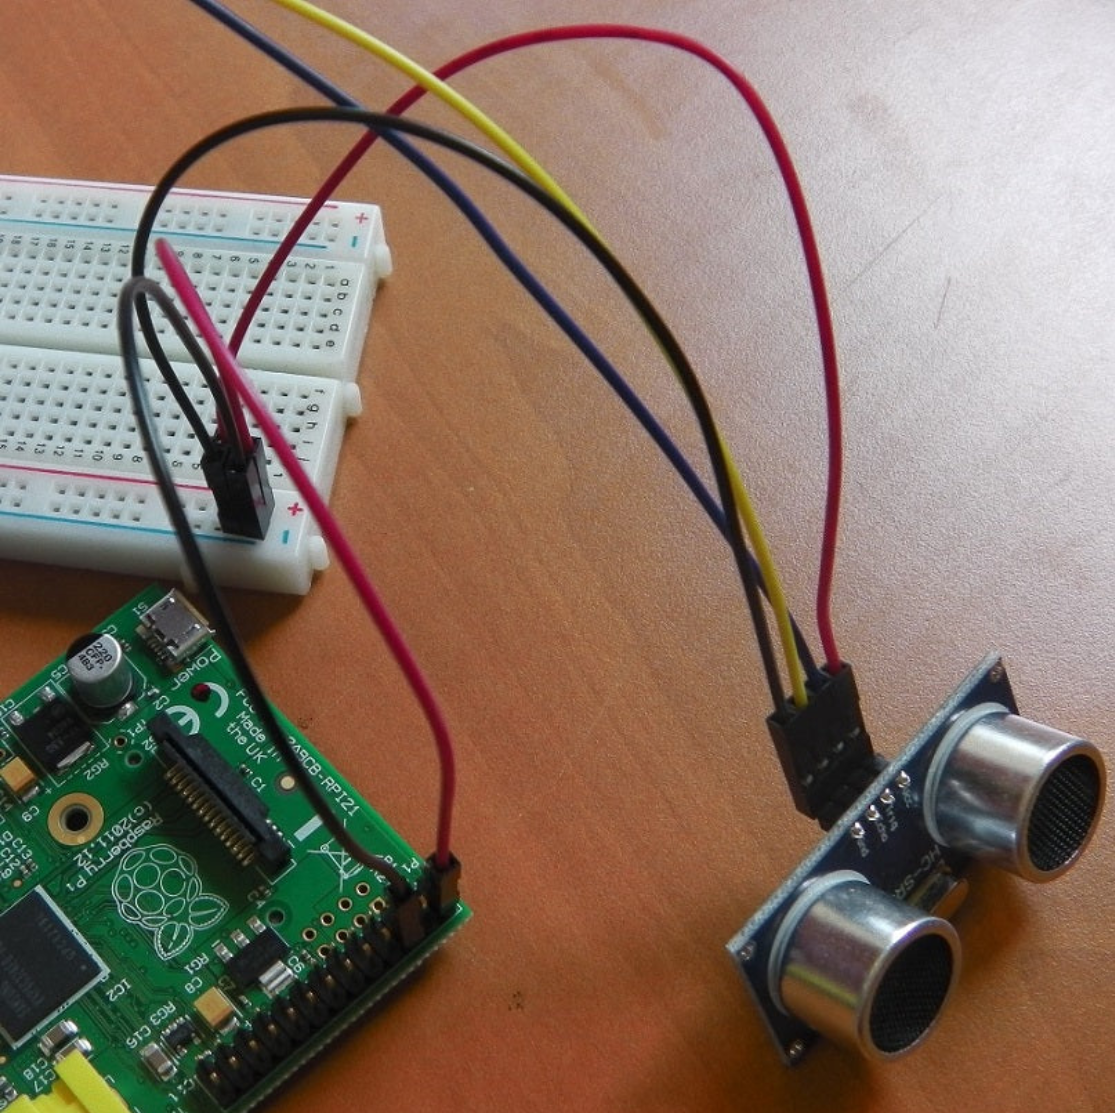
\includegraphics[width=14cm]{screenshots/7.png}\\
		      \caption{Подключение контактов 5В и GND к макетной плате}
	      \end{figure}
	\item Вставляем TRIG в пустую шину и подключаем эту шину к GPIO 23.
	      \begin{figure}[H]
		      \centering
		      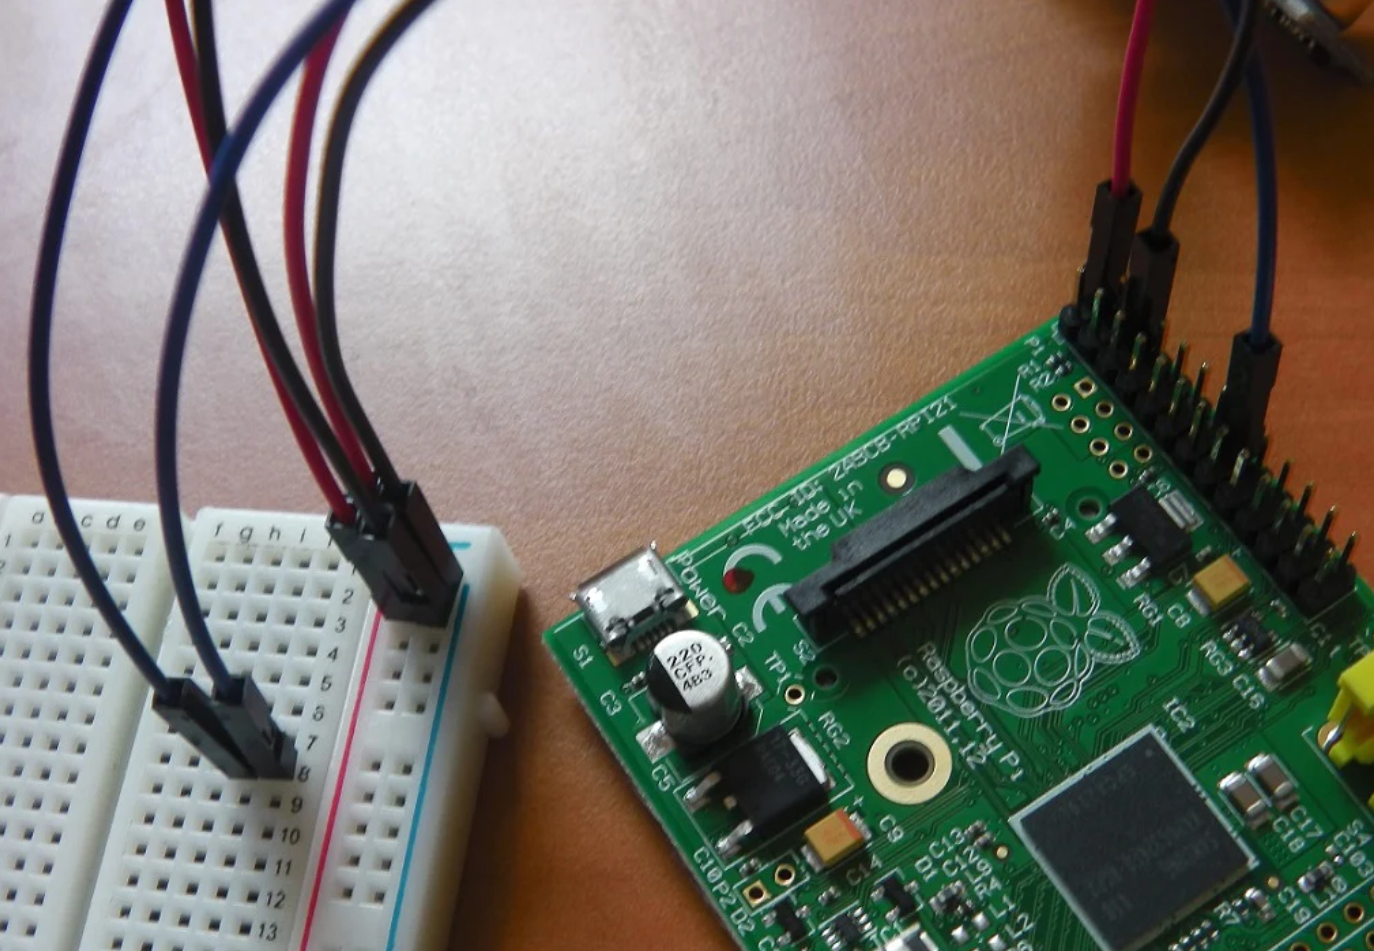
\includegraphics[width=14cm]{screenshots/8.png}\\
		      \caption{Подключение TRIG}
	      \end{figure}
	\item Подключаем ECHO к пустой шине, соединяем другую пустую шину с первой с помощью $R_1$ ($1 \text{k}\Omega$).
	\item Соединяем шину c $R_1$ с шиной GND с помощью резистора $R_2$ ($2 \text{k}\Omega$), оставив пространство между двумя резисторами.
	      \begin{figure}[H]
		      \centering
		      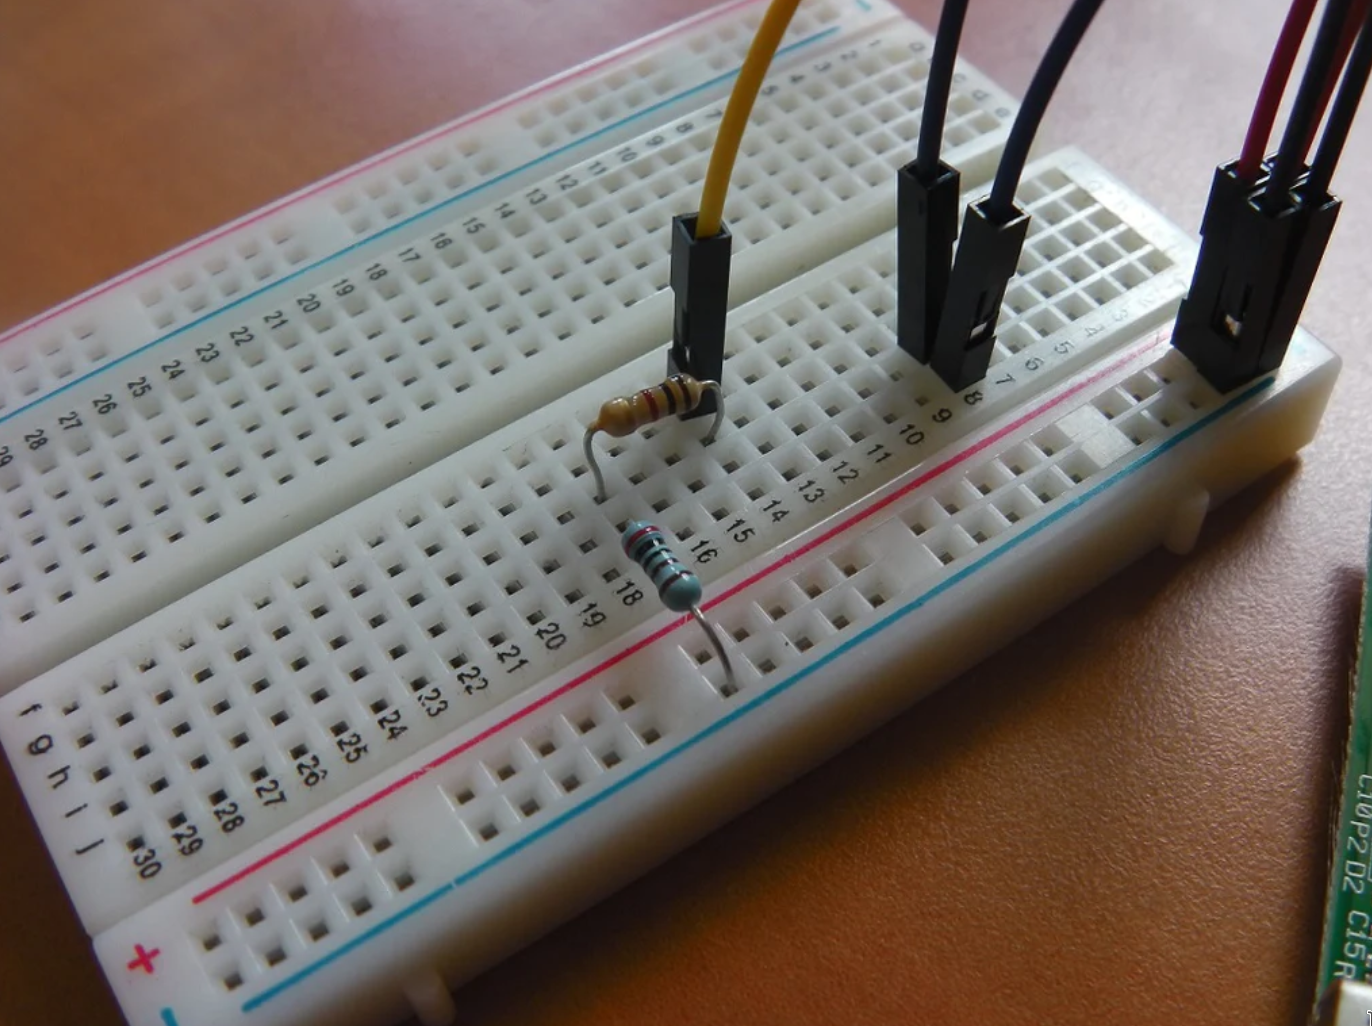
\includegraphics[width=14cm]{screenshots/9.png}\\
		      \caption{Подключение резисторов к макетной плате}
	      \end{figure}
	\item Подключаем GPIO 24 к шине с $R_1$. Этот вывод GPIO должен располагаться \textit{между} $R_1$ и $R_2$.
	      \begin{figure}[H]
		      \centering
		      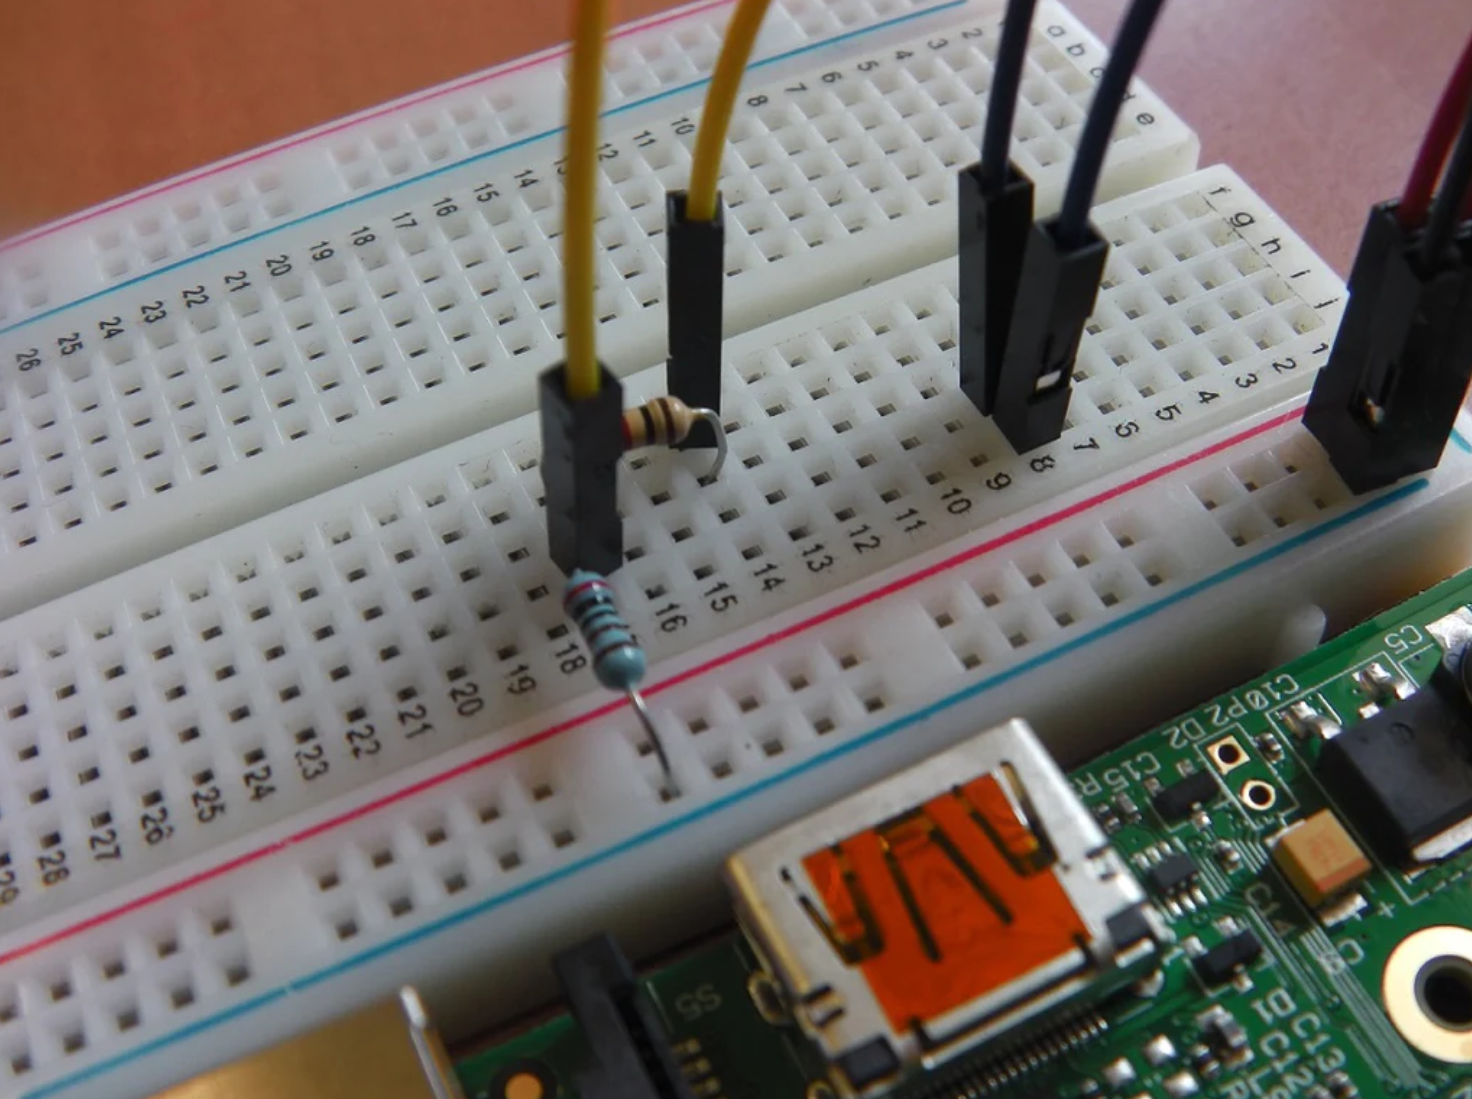
\includegraphics[width=14cm]{screenshots/10.png}\\
		      \caption{Подключение GPIO 24}
	      \end{figure}
	\item Наш датчик HC-SR04 оказывается подключенным к Raspberry Pi.
	      \begin{figure}[H]
		      \centering
		      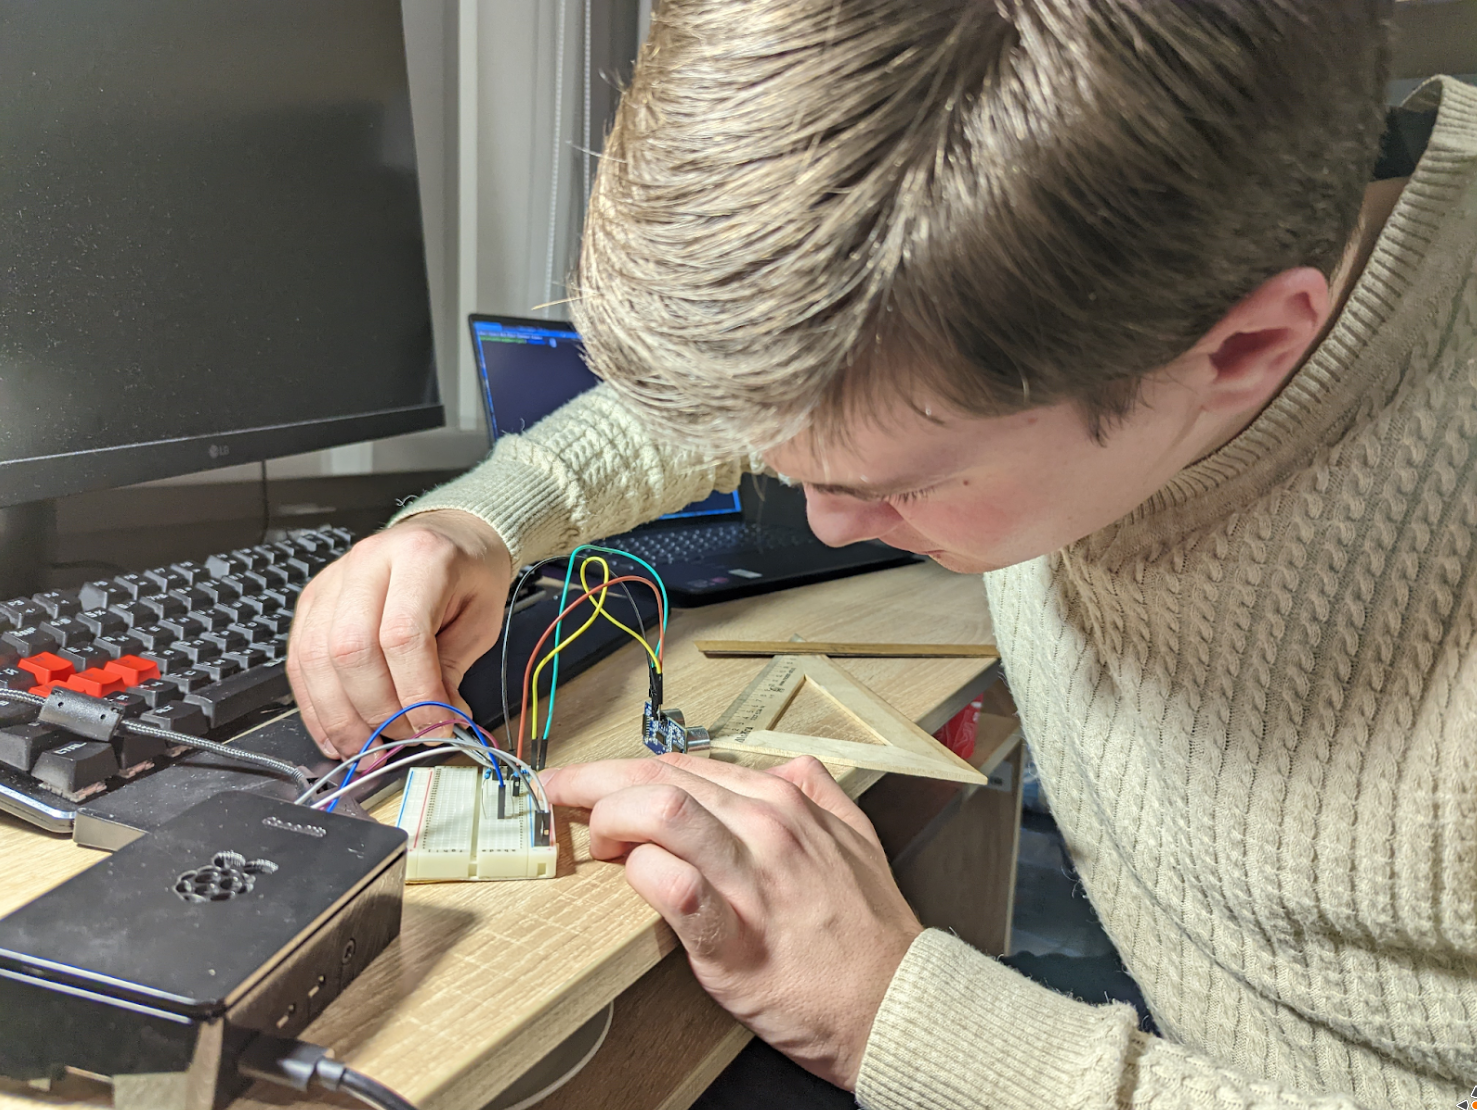
\includegraphics[width=14cm]{screenshots/11.png}\\
		      \caption{Финал подключения}
	      \end{figure}
\end{enumerate}

\newpage
\section{Программная часть}

Теперь, когда мы подключили наш ультразвуковой датчик, нам нужно написать Python скрипт для определения расстояния.

Выход ультразвукового датчика ECHO будет всегда иметь низкий уровень сигнала 5В, если только он не сработал. Поэтому нам нужно установить один контакт GPIO в качестве выхода для срабатывания датчика и один в качестве входа для обнаружения изменения напряжения ECHO.

Датчику HC-SR04 требуется короткий импульс длительностью 10 мкс для запуска модуля, который заставит датчик запустить программу измерения дальности (8 ультразвуковых импульсов с частотой 40 кГц) для получения эхо-ответа. Итак, чтобы создать наш триггерный импульс, мы устанавливаем триггерный контакт в высокий уровень на 10 мкс, а затем снова устанавливаем его в низкий уровень.

Как только сигнал получен, значение ECHO изменяется с низкого (логический ноль) на высокое (логическая единица), и сигнал остается высоким на протяжении всего эхо-импульса. Поэтому нам также нужна последняя высокая метка времени для ECHO (т.е. тот момент времени, когда в последний раз сигнал был высоким).

Теперь мы можем вычислить разницу между двумя записанными метками времени и, следовательно, получить длительность импульса.

Учитывая время, необходимое сигналу для прохождения к объекту и обратно, мы можем рассчитать расстояние.

Скорость звука варьируется в зависимости от среды, через которую он проходит, а также от температуры этой среды. Однако, физики рассчитали скорость звука на уровня моря, которую мы можем взять за основу:
$$v_{\text{звука}} = 343 \frac{\text{м}}{\text{c}}$$

Нам также нужно будет разделить наше время на два, потому что сейчас мы имеем время, которое требуется ультразвуковому импульсу для прохождения расстояния до объекта и обратно.

Также, для повышения точности будем делать по три замера и выводить на экран среднее арифметическое. Выводы будем осуществлять в автоматическом режиме раз в секунду.

Исходный текст программы представлен в конце отчета.

\newpage
\section{Raspberry Pi 4B. Удаленное управление через SSH}

SSH (Secure Shell) - протокол передачи данных по сети, позволяющий производить удаленное управление операционной системой через шифрованное соединение, а также передавать файлы, транслировать видео и аудио потоки и сжимать передаваемые данные на лету. Говоря простым языком, SSH позволяет нам установить соединение, через которое можно запустить на компьютере терминал для выполнения консольных команд на другом компьютере.

Для демонстрации мы используем SSH-клиент JuiceSSH для Android.

\newpage
\section{Результаты работы}

\begin{figure}[H]
	\centering
	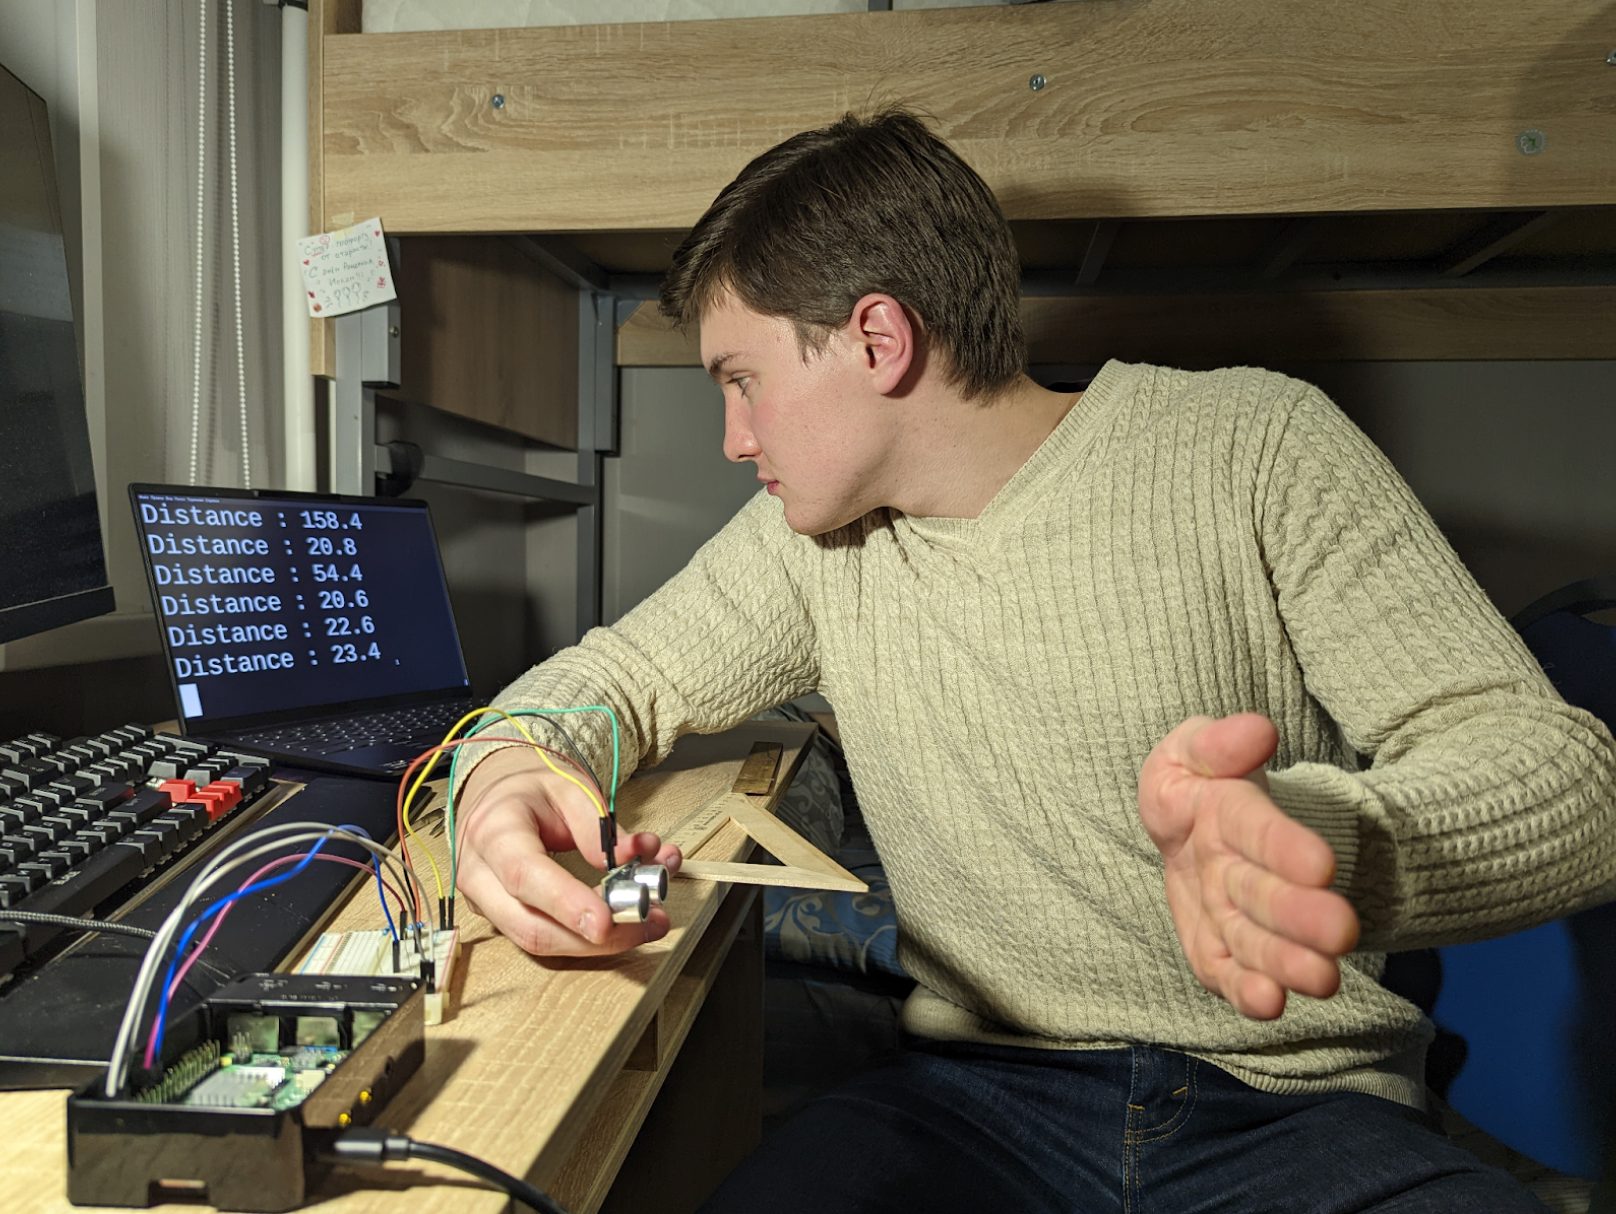
\includegraphics[width=15cm]{screenshots/12.png}\\
	\caption{Тестирование схемы}
\end{figure}

В ходе тестирования было проведено 4 измерения: 2 на малом расстоянии, 1 на среднем расстоянии и 1
на большом расстоянии. Измерения проводились в стандартном коридоре, в качестве отражающей поверхности на малом расстоянии использовалась упаковка туалетной бумаги, а в тестах на среднем
и большом расстоянии - стена.

\begin{itemize}
	\item На малом расстоянии (100мм) прибор в среднем показывал результат 103мм.
	\item На малом расстоянии (500мм) прибор в среднем показывал результат 503мм.
	\item На среднем расстоянии (1000мм) прибор вначале показывал заниженные результаты при измерении от пола, что связано с отражением ультразвука от данной поверхности. Однако при измерении с возвышенности результат вновь стал корректным, прибор показывал результат 1015мм.
	\item На большом расстоянии (3000мм) прибор показывал данные значительно меньше фактического расстояния (1300мм). Данный эффект объясняется тем, что в данном тесте расстояние до боковых стен являлось значительно меньше расстояния до объекта. Так как в таком случае звук от боковых стен возвращался быстрее, чем от объекта, то выводимое расстояние было меньше фактического.
\end{itemize}

Также, в ходе тестирования был измерен фактический угол работы датчика. В исходном положении, датчик находился под углом $0^\circ$ к нормали. Далее, датчик постепенно отклоняли вплоть до положения, в котором измеряемое датчиком расстояние перестало соответствовать реальному.
Выяснилось, что максимальный угол, при котором датчик продолжает показывать расстояние до плоскости, к  которой проведена нормаль, составляет около $40^\circ$, что является фактическим углом работы датчика. При этом производителем заявлен эффективный угол в $15^\circ$.
\newpage
\section{Вывод}

В ходе работы нами был разработан ультразвуковой дальномер с использованием Raspberry Pi и ультразвукового датчика HC-SR04. Для этого потребовалось спроектировать схему подключения, а также разработать программный код на языке Python для взаимодействия с датчиком по GPIO.

В ходе тестирования выяснилось, что проведение измерений в замкнутых пространствах невозможно из-за отражения звуковых волн от прочих стен помещения. Однако, в условиях близких к условиям открытого пространства, то есть когда расстояние до объекта меньше расстояния до прочих отражающих поверхностей, тесты показали удовлетворительный результат.

\newpage
\section{Исходные тексты программ}

\subsection{main.py}
\normalsize
\inputminted[frame=single]{python}{../src/main.py}
\Large
\newpage
\section{Список литературы и электронных источников}

\begin{itemize}
	\item https://vk.cc/ciHt99 - установка Linux на RaspberryPi.
	\item https://vk.cc/ciHteo - подключение модуля к RaspberryPi.
	\item https://vk.cc/ciHtk8 - обработка данных с модуля.
	\item https://vk.cc/ciHtqu - подключение к RaspberryPi по SSH.
\end{itemize}

\end{document}
